
\documentclass{jtetiproposalskripsi}

%-----------------------------------------------------------------
%Disini awal masukan untuk data proposal skripsi
%-----------------------------------------------------------------
\titleind{Aplikasi Penggajian Pegawai Berbasis WEB}
\fullname{NADIYATUL AYNUN JARIYAH}

\idnum{1200631020}

\approvaldate{3 Januari 2015}

\degree{Diploma Tiga Komputer}

\yearsubmit{2015}

\program{Manajemen Informatika}

\headprogram{Sarjiya, S.T., M.T., Ph.D.}

\dept{Teknik Manajemen Informatika}

\firstsupervisor{Victor Wahanggara, S.Kom}
\firstnip{1203716}

\secondsupervisor{Yeni dwi Rahayu, M.Kom}
\secondnip{1977 0131 2002 12 1 003}


%-----------------------------------------------------------------
%Disini akhir masukan untuk data proposal skripsi
%-----------------------------------------------------------------

\begin{document}

\cover

\approvalpage

%-----------------------------------------------------------------
%Disini akhir masukan untuk muka skripsi
%-----------------------------------------------------------------

%-----------------------------------------------------------------
%Disini awal masukan Intisari
%-----------------------------------------------------------------
\begin{abstractind}
Seiring dengan perkembangan teknologi khususnya teknologi informasi yang begitu pesat, maka dalam manajemen pendidikian dituntut untuk bisa meningkatkan mutunya dalam dunia teknologi. Mengapa demikian, karena agar kebutuhan manajemen dalam pendidikan dapat berjalan mengikuti alur teknologi yang ada.
Aplikasi Penggajian Pegawai Yayasan Paud Terpadu Al-Mahrus hanya mengkaji tentang data gaji pegawai, data pinjaman yang dilakukan oleh para pengajar, data absensi dari pegawai, data pegawai, serta data lembur pegawai. Aplikasi Penggajian Pegawai Di Yayasan Paud Terpadu Al-Mahrus tidak mengkaji tentang data siswa maupun data pembayaran siswa di lembaga sekolah tersebut.

Dengan adanya program penggajian, maka lembaga sekolah terutama manajemen administrasi tidak perlu lagi mencatat jumlah gaji dari setiap pengajar dan juga tidak perlu lagi memberikan gaji secara tunai. Karna sistem pemberian gaji yaitu mengirim pada setiap rekening para pengajar.


\bigskip
\textbf{Kata kunci} : \emph{Aplikasi Penggajian Pegawai Berbasis Web}.
\end{abstractind}
%-----------------------------------------------------------------
%Disini akhir masukan Intisari
%-----------------------------------------------------------------

\tableofcontents
\addcontentsline{toc}{chapter}{DAFTAR ISI}
\selectlanguage{bahasa}\clearpage\pagenumbering{arabic}\setcounter{page}{1}

%-----------------------------------------------------------------
%Disini awal masukan untuk Bab
%-----------------------------------------------------------------
\chapter{LATAR BELAKANG}

\section{Latar Belakang Masalah}
Seiring dengan perkembangan teknologi khususnya teknologi informasi yang begitu pesat, maka dalam manajemen pendidikian dituntut untuk bisa meningkatkan mutunya dalam dunia teknologi. Mengapa demikian, karena agar kebutuhan manajemen dalam pendidikan dapat berjalan mengikuti alur teknologi yang ada. Selain itu, manajemen pendidikan juga dituntut untuk dapat memberikan sebuah informasi yang mudah untuk di akses di berbagai tempat. Disinilah informasi dan tegnilogi memegang peranan penting, karena informasi dan teknologi dibutuhkan oleh semua pihak. Baik berupa individu maupun organisasi, lembaga atau perusahaan. Setiap informasi yang didapat berguna untuk mendukung pengambilan keputusan yang tepat. 

Peranan teknologi komputer di era globalisasi sekarang ini sangat penting dalam pengolahan informasi di perusahaan. Karena dengan menggunakan pengolahan informasi yang berbasis komputer akan mampu menghasilkan suatu informasi yang tepat, akurat dan bermanfaat bagi organisasi, lembaga maupun perusahaan. Pada Yayasan Paud Terpadu Al-Mahrus,masalah pembayaran gaji merupakan masalah yang sangat penting. Karena gaji merupakan wujud imbalan yang diberikan lembaga sekolah kepada para pegawaiyang telah memberikan tenaganya untuk memberikan pelajaran berbagai ilmu dalam lingkupsekolah tersebut. Gaji merupakan salah satu unsur penting bagi lembaga sekolah. Karena jika gaji yang diberikan terlalu kecil maka kinerja para pegawaitidak akan maksimal. Untuk itu diperlukan adanya sistem elektronik (komputer) untuk mengolah data yang tepat dan cepat. Karenadengan menggunakan sistem secara manual bagian administrasi tidak dapat berjalan secara efektif dan efisien sehingga dapat mengacaukan data dan memperlambat kinerja para pegawainya. 

Dengan adanya program penggajian, maka lembaga sekolah terutama manajemen administrasi tidak perlu lagi mencatat jumlah gaji dari setiap pengajar dan juga tidak perlu lagi memberikan gaji secara tunai. Karna sistem pemberian gaji yaitu mengirim pada setiap rekening para pengajar. Disamping itu juga, para pengajar tidak perlu datang langsung pada manajemen administrasi untuk mengetahui jumlah gaji setiap pengajar. Melalui aplikasi penggajian ini semua akan dipermudah dengan satu akses.
Dalam hal ini penggunaan perangkat komputer dapat digunakan sebagai alat bantu dalam mengelola setiap transaksi yang ada. Sehingga dengan penulisan tugas akhir ini maka penulis tertarik untuk membuat program penggajian pegawai di Yayasan Paud Terpadu Al-Mahrus. Penulis memilih judul: “ Aplikasi Penggajian Pegawai Di Yayasan Paud Terpadu Al-MahrusBerbasis Web “



\section{Rumusan Masalah}
Berdasarkan latar belakang di atas, maka rumusan masalah yang akan dikaji oleh penulis dalam Tugas Akhir ini adalah bagaimana cara merancang aplikasi penggajian sehingga dapat mempermudah dalam memberikan informasi dan menyimpan data.
\begin{itemize}
\item[1.]BagaimanaPerancanganAplikasi Penggajian Pegawai Di Yayasan Paud Terpadu Al-Mahrus.
\item[2.]BagaimanapengujianPerancanganAplikasi Penggajian Pegawai Di Yayasan Paud Terpadu Al-Mahrus.
\item[3.]BagaimanaevaluasiPerancanganAplikasi Penggajian Pegawai Di Yayasan Paud Terpadu Al-Mahrus.
\end{itemize}

\section{Batasan Masalah}

Aplikasi Penggajian Pegawai Yayasan Paud Terpadu Al-Mahrus hanya mengkaji tentang data gaji pegawai, data pinjaman yang dilakukan oleh para pengajar, data absensi dari pegawai, data pegawai, serta data lembur pegawai.Aplikasi Penggajian Pegawai Di Yayasan Paud Terpadu Al-Mahrus tidak mengkaji tentang data siswa maupun data pembayaran siswa di lembaga sekolah tersebut.

\section{Tujuan}
Penelitian ini memiliki tujuan memperbaiki sistem lama, yang secara manual dan mengganti dengan sistem baru, berjalan dengan menggunakan teknologi informasi melalui komputer. Penggantian sistem ini bertujuan Dapat menghemat waktu, dapat dengan mudah di akses kapan saja.


\section{Manfaat Penelitian}
Manfaat dari dibuatnya sistem ini yaitu :
\begin{itemize}
\item[1.]Dapat menghemat waktu.
\item[2.]Dapat dengan mudah  di akses kapan saja.
\item[3.]Mempermudah pegawai untuk mendapatkan informasi tentang data gaji.
\item[4.]Dan mengumpulkan serta menyajikan beberapa data dalam satu aplikasi. 
\end{itemize}

%-------------------------------------------------------------------------------
\chapter{TINJAUAN PUSTAKA}               
\section{Tinjauan Aplikasi}
\subsection{Pengertian Sistem}
Terdapat dua kelompok pendekatan di dalam pendefinisian sistem, yaitu kelompok yang menekankan pada prosedur dan kelompok yang menekankan pada elemen atau komponennya. Pendekatan yang menekankan pada prosedur mendefinisikan sistem sebagai suatu jaringan kerja dari prosedur-prosedur yang saling berhubungan. Sedangkan pendekatan sistem yang lebih menekankan pada elemen atau komponen mendefinisikan sistem sebagai kumpulan dari elemen-elemen yang berinteraksi untuk mencapai suatu tujuan tertentu. Kedua kelompok definisi ini adalah benar dan tidak bertentangan, yang berbeda adalah cara pendekatannya saja.

	Secara sederhana sistem dapat diartikan sebagai suatu kumpulan atau himpunan dari unsur, komponen atau variabel-variabel yang terorganisasi, saling berinteraksi, saling tergantung satu sama lain dan terpadu.
	Sistem adalah sekelompok elemen yang terintegrasi dengan maksud yang sama untuk mencapai suatu tujuan.( McLeod dalam Al-Bahra, 2005)
	
menyatakan bahwa suatu sistem adalah sebuah perangkat elemen-elemen yang terintegrasi dengan maksud yang sama untuk mencapai tujuan bersama.( Robert G. Murdick dalam Al-Bahra,2005).
	Pendekatan sistem yang lebih menekankan pada prosedur di definisikan bahwa sistem yaitu suatu jaringan kerja dari prosedur-prosedur yang saling berhubungan, berkumpul bersama-sama untuk melakukan suatu kegiatan atau menyelesaikan suatu sasaran tertentu 

\subsection{Pengertian informasi}
Informasi merupakan proses lebih lanjut dari data yang sudah memiliki nilai tambah. Istilah informasi seringkali tidak tepat pemakaiannya. Informasi dapat merujuk ke suatu data mentah, data tersusun, kapasitas sebuah saluran komunikasi, dan lain sebagainya. Suatu sistem yang kekurangan informasi akan menjadi lemah dan akhirnya berakhir.

Informasi adalah data yang diklasifikasikan atau diolah atau diiterprestasikan untuk digunakan dalam proses pengambilan keputusan. Sistem pengolahan informasi akan mengolah data menjadi informasi atau mengolah data dari bentuk tidak berguna menjadi berguna bagi yang menerimanya. 

Informasi merupakan data yang telah di olah menjadi bentuk yang lebih berarti dan berguna bagi penerimanya untuk mengambil keputusan masa kini maupun masa datang.( Gordon B. Davis dalam Al-Bahra,2005)  
Sumber informasi adalah data. Data adalah kenyataan yang menggambarkan kejadian dan kesatuan nyata. Kejadian (event) adalah suatu yang terjadi pada saat tertentu. Informasi diperoleh dari data-data mentah diproses atau diolah.

Agar informasi yang dihasilkan lebih berharga, maka informasi harus memenuhi kriteria berikut :

\begin{itemize}

\item[1.] Informasi harus akurat, sehungga mendukung pihak manajemen dalam mengambil keputusan.
\item[2.] Informasi harus relevan, benar-benar terasa manfaatnya bagi yang membutuhkan.
\item[3.] Informasi harus tepat waktu, sehingga tidak ada keterlambatan pada saat yang dibutuhkan.
\end{itemize}

Dari keterangan diatas, sesuatu dapat dikatakan informasi apabila suatu data sudah di olah menjadi data yang berharga dan bermanfaat dimata penggunanya. Informasi dikatakan bernilai jika manfaat lebih besar dari pada di banding biaya uantuk mendapatkannya. Informasi dikatakan berkualitas apabila memenuhi tiga criteria yaitu Akurat ( Accurate ), tepat pada waktunya ( Timeliness ), relevan ( Relevanse ). (John Burch , Gary Grudnitski dalam Al-Bahra,2005)


\subsection{Konsep Sistem Informasi}
Sistem informasi adalah suatu sistem di dalam suatu organisasi yang mempertemukan kebutuhan pengolahan transaksi harian, mendukung operasi, bersifat manajerial dan strategi dari suatu organisasi dan dapat menyediakan pihak luar tertentu dengan laporan-laporan yang ditentukan. (Robert A. Leitch dan K. Roscoe Davis dalam Hartono,1999)

Sistem informasi adalah suatu sistem di dalam suatu organisasi yang merupakan kombinasi dari orang-orang, fasilitas, teknologi, media, prosedur-prosedur, dan pengendalian yang ditujukan untuk mendapatkan jalur komunikasi penting, memproses tipe transaksi rutin tertentu, memberi sinyal kepada manajemen dan yang lainnya terhadap kejadian-kejadian internal dan eksternal yang penting dan menyediakan suatu dasar informasi untuk pengambilan keputusan yang cerdik (Hartono, 1999).


\subsection{Tinjauan Database}
Database adalah kumpulan file-file yang mempunyai kaitan antara satu file dengan file yang lain sehingga membentuk satu bangunan data untuk menginformasikan satu perusahaan, instansi tersebut dalam batasan tertentu. Bila terdapat file yang tidak dapat dipadukan atau dihubungkan dengan file yang lainnya berarti file tersebut bukanlah kelompok dari satu database, akan membentuk satu database tersendiri. (Kristanto, 1994).

Basis data (database) merupakan kumpulan dari data yang saling berhubungan satu dengan yang lainnya, tersimpan di perangkat keras komputer dan digunakan perangkat lunak untuk memanipulasinya. Database merupakan salah satu komponen yang penting dalam sistem informasi, karena merupakan basis dalam menyediakan informasi bagi para pemakai. (Hartono,1999).

Basis data (database) merupakan kumpulan dari data yang saling berhubungan satu dengan yang lainnya, di simpanan luar komputer dan menggunakan perangkat lunak tertentu untuk memanipulasinya. Database merupakan salah  satu komponen yang penting di sistem informasi, karena berfungsi sebagai  basis penyedia informasi bagi para pemakainya. Penerapan database dalam  sistem informasi disebut dengan database system. Sistem basis data (database system) ini adalah suatu sistem informasi yang mengintegrasikan kumpulan dari data yang saling berhubungan satu dengan lainnya dan membuatnya tersedia untuk beberapa aplikasi yang bermacam-macam di dalam  suatu organisasi. Tujuan dari desain database adalah untuk menentukan data-data yang dibutuhkan dalam sistem, sehingga informasi yang dihasilkan dapat terpenuhi dengan baik. 

\subsection{Sistem Informasi Penggajian}
Gaji adalah balas jasa atas faktor produksi tenaga kerja yang tidak dipengaruhi oleh produksi atau pembayaran atas penyerahan jasa yang dilakukan oleh para karyawan. Gaji lebih banyak dipakai untuk para karyawan yang dibayar secara bulanan. Sedangkan upah adalah bayaran yang diberikan untuk para pekerja harian, diberikan pada para pekerja dan dibayarkan berdasarkan hari kerja.

	Beberapa pendapat mengenai penggajian :
	
\begin{itemize}
\item[1.] Mulyadi (1989)
“Gaji adalah pembayaran atas penyerahan jasa yang dilakukan 	oleh karyawan baik yang mempunyai jabatan  maupun karyawan  pelaksana”.
\item[2.] Rokmulyati (1983)
”Penggajian adalah suatu proses pemberian motivasi kepada karyawan yang dilakukan secara periodik”.
	Penghasilan yang didapat oleh seorang karyawan terdiri atas :

\item[a.] Gaji Pokok
Gaji pokok adalah besarnya gaji yang diberikan kepada pegawai sesuai dengan jasanya bekerja untuk prusahaan yang sudah ditetapkan gaji pokok minimum pada waktu pertama kali karyawan tersebut bekerja.
 
Keterangan :
Yang dimaksud jam kerja disini adalah jumlah jam kerja para guru selama satu bulan. Dan besar nominal berdasarkan keputusan lembaga pendidikan tersebut.
Gaji pokok ini hanya diberikan kepada para guru saja. Sedangkan untuk para pegawai yang selain guru tidak mendapatkan gaji pokok.

\item[b.] Insentive
•	Uang transport
 
Keterangan :
Total jam kerja dihitung berdasarkan jumlah jam kerja pegawai selama satu  bulan. Dan besarnya upah transport per jam dihitung berdasarkan ketentuan perusahaan.

\item[c.] Tunjangan
		Tunjangan diberikan kepada setiap pegawai yang biasanya diberikan setiap penggajian. Tunjangan yang diberikan para pegawai adalah tunjangan Jabatan.
		Tunjangan jabatan Adalah tunjangan yang memiliki jabatan di lembaga pendidikan tersebut dan besar nominal tunjangan dibedakan berdasarkan jabatannya.

\item[d.]	Potongan
Adapun jenis potongan yang ada  adalah sebagai berikut :
a.	Potongan Iuran Guru
Potongan ini diambil dari gaji kotor yang besarnya menurut ketentuan lembaga pendidikan tersebut.
b.	Potongan Lazis
Setiap pendidikan yang dibawah naungan Muhammadiyah, tiap pegawai yang bekerja diwajibkan untuk membayar iuran kepada lazis. 
5.	Presensi
Presensi adalah tanda kehadiran pegawai sebelum melakukan aktivitasnya yaitu bekerja di sebuah instansi. Yang dicatat diawal pegawai ketika memulai pekerjaanya dan mencatat akhir pegawai untuk menyelesaikan tugasnya. Karena dari presensi itulah dapat diketahui jumlah jam kerja tiap pegawai untuk melakukan proses penggajian.


\end{itemize}


\subsection{Tinjauan Singkat Perangkat Lunak MySql}
MySQL adalah sebuah server database SQL multiuser dan multi-threaded. SQL  sendiri  adalah  salah  satu  bahasa  database  yang  paling  populer  di  dunia. Implementasi  program  server  database  ini  adalah  program  daemon  'mysqld'  dan beberapa program lain serta beberapa pustaka.
MySQL dibuat oleh TcX dan  telah dipercaya mengelola  sistem dengan 40  buah database berisi 10,000  tabel dan 500 di antaranya memiliki 7  juta baris (kira-kira 100  gigabyte  data).  Database  ini  dibuat  untuk  keperluan  sistem  database  yang cepat, handal dan mudah digunakan. Walaupun memiliki kemampuan yang cukup baik, MySQL  untuk  sistem  operasi  Unix  bersifat  freeware,  dan  terdapat  versi shareware untuk sistem operasi windows. Menurut pembuatnya, MySQL disebut seperti "my-ess-que-ell" dan bukan my-sequel ! 
Sebagaimana database sistem yang  lain, dalam SQL  juga dikenal hierarki server  dengan  database-database.  Tiap-tiap  database memiliki  tabel-tabel.  Tiap-tiap tabel memiliki field-field.  Umumnya  informasi  tersimpan dalam  tabel –  tabel yang secara  logik merupakan struktur 2 dimensi    terdiri atas baris dan kolom.Field-field  tersebut dapat berupa data seperti int , realm char, date, time dan lainnya.  
SQL  tidak  memiliki  fasilitas  pemrograman  yang  lengkap,  tidak  ada looping ataupun percabangan  ,misalnya. Sehingga untuk menutupi kelemahan  ini perlu digabung dengan bahasa pemrograman semisal C.   (www.mysql.com)


\subsection{Java dan Neat Beans}
Java merupakan pemrograman yang dikembangkan oleh Sun Microsystem, dan dirancang sedemikian rupa agar program yang dibuat menggunakan Java dapat berjalan pada semua platform. Untuk beragam aplikasi yang dibuat dengan bahasa Java, Java dipaketkan dalam edisi-edisi berikut:

\begin{itemize}
\item[1.] Java   2   Standar   Edition   (J2SE)
J2SE  menyediakan   lingkungan pengembangan yang kaya fitur,  stabil,  aman,  dan  cross-platform. Edisi ini mendukung konektivitas  basis  data,   rancangan  user   interface,  masukkan/ keluaran (input/output), dan pemrograman jaringan (network programming), dan termasuk sebagai paket-paket dasar bahasa Java.
\item[2.] Java   2   Enterpise   Edition   (J2EE)
J2EE   menyediakan   tempat   untuk membangun   dan  menjalankan  multitier   enterprise   editions.   J2EE   berisi paket paket di J2SE ditambah paket-paket untuk mendukung pengembangan Enterprise JavaBeans,  Java Servlets,  JavaServer Pages,  XML, dan kendali transaksi yang fleksibel.
\item[3.] Java 2 Micro Edition (J2ME)
J2ME selain menyedikan bahasa Java yang sama, unggul dalam portabilitas (kemampuan dapat dijalankan dimanapun), safe   network   delivery,   seperti   J2SE   dan   J2EE.   Aplikasi-aplikasi   dapat diskalakan (dimampukan) agar dapat bekerja dengan J2SE dan J2EE. J2ME adalah untuk beragam  consumer  electronic product,  seperti  pager,  smart  card, cell phone, handheld PDA, dan set-top box.
Ada   3   kombinasi   kunci   yang   membuat   Java   menjadi   teknologi   yang   secara fundamental berbeda dari yang lain, yang ada saat ini. Pertama,  semua orang dapat menggunakan  applet  yang   kecil,   aman,   dinamik,   lintas-platform,   aktif,   dan   siap dijalankan di   jaringan  sejak awal.  Kedua,   Java adalah bahasa pemrograman yang ampuh,  memiliki kekuatan desain berorientasi objek dengan sintaks yang sederhana dan mudah dikenal.  Ketiga,  Java adalah kumpulan  class object  yang ampuh,  yang melayani  programmer  dengan uraian yang jelas untuk banyak fungsi sistem umum, seperti pembuatan window, penggunaan jaringan, dan input/ output.

\end{itemize}


Beberapa Fitur-fitur Penting Dalam Bahasa Java

\begin{itemize}
\item[-] Bahasa sederhana
Java dirancang untuk mudah dipelajari dan digunakan dengan secara efektif. Java tidak mendukung fitur-fitur rumit seperti:

\item[1.] Explicit pointer manipulation
\item[2.] Implicit type casting
\item[3.] Structures atau union
\item[4.] Operator overloading
\item[5.] Templates
\item[6.] Header files
\item[7.] Multiple inheritance
\end{itemize}

Rancangan bahasa Java telah berdasar teknologi yang telah terbukti dan dikembangkan di bahasa-bahasa pemrograman lainnya.

*	Bahasa berororientasi objek
Java   bukan   turunan   langsung   dari   bahasa   pemrograman  manapun,   juga   sama sekali   tidak kompatibel  dengan semuanya.  Model  objek Java adalah sederhana dan  mudah  dikembangkan,   namun   sejalan  dengan   itu,  nilangan   dan  tipe   data sederhana lain dianggap sebagai non-objek berkinerja tinggi.OOP (object oriented programming) adalah cara ampuh dalam pengorganisasian dan   pengembangan   perangkat   lunak.   Pada  OOP,   program  komputer   sebagai sekelompok objek yang  saling berinteraksi.  Objek-objek  ini  ada  secara  secara independent yang mempunyai aturan-aturan berkomunikasi dengan objek lain dan untuk memerinthakan objek lain guna meminta informasi tertentu atau meminta objek lain mengerjakan sesuatu.

*	Bahasa statically typed
Semua objek dideklarasikan terlebih dahulu sebelu m digunakan. Melalui fitur ini kode program lebih dapat dioptmasi untuk menghasilkanprogram berkinerja tinggi.

*	Bahasa dikompilasi
Sebelum   menjalankan   program   di   bahasa   Java,   program   dikompilasi menggunakan Java Compiler. Kompilais akan menghasilkan file “bytecode” yang serupa fungsinya dengan file kode mesin.  Program “bytecode” yang dihasilkan dapat di eksekusi di sembarang Java Interpreter.  Java Interpreter  membaca file “bytecode” dan menterjemahkan perintah “bytecode” menjadi  perintah-perintah bahasa mesin yang dapat di eksekusi mesin.

*	Bahasa yang aman
Java menggunakan model pengamanan 3 lapis untuk melindungi sistem dari Untrusted Java Code.
	 Bytecode   verifier  membaca  bytecode  sebelum   dijalankan   dan menjamin bytecode memenuhi aturan-aturan dasar bahasa Java Class loader menangani pemuatan kelas Java ke runtime interpreter. Manajer   keamanan  menangani   keamanan   tingkat   aplikasi   dengan mengendalikan   apakah   program  berhak  mengakses   sumber   daya seperti   sistem  file,  port  jaringan,   proses   eksternal   dan   system windowing.
Selain itu Java menyediakan beragam teknik pengaman, yaitu:
\begin{itemize}

\item[1.] Bahasa dirancang untuk mempersulit eksekusi kode perusak
\item[2.] Program Java dikompilasi menjadi serangkaian bytecode.
\item[3.] Java mempunyai pengamanan terhadap applet.

\end{itemize}

*	Bahasa independen terhadap platform
Platform independence merupakan kemampuan program bekerja di sistem operasi atau sistem komputer berbeda. Bahasa Java adalah bahasa yang secara sempurna tidak bergantung platform.

*   Bahasa multithreading
Thread adalah menyatakan program komputer melakukan lebih dari satu tugas di satu  Waktu   yang   sama.   Java   menyediakan   kakas   untuk   menulis   program multithread,  program mempunyai   lebih dari  1  thread  eksekusi  pada  saat  yang sama   sehingga   memungkinkan   program   menagani   beberapa   tugas   secara konkuren.

*   Bahasa yang didukung garbage collector
Artinya,   program   tidak   perlu   menghapus   sendiri   objek-objek   yang   tidak digunakan   lagi.   Fasilitas   ini   mengurangi   beban   pengelolaan   memori   oleh pemrogram dan mengurangi atau mengeliminasi sumber kesalahan terbesar yang terdapat di bahasa yang memungkinkanalokasi dinamis.



%-------------------------------------------------------------------------------
\chapter{METODE PENELITIAN}

\section{Flowchart Metode Penelitian}
\begin{figure}[h]
\centering 
 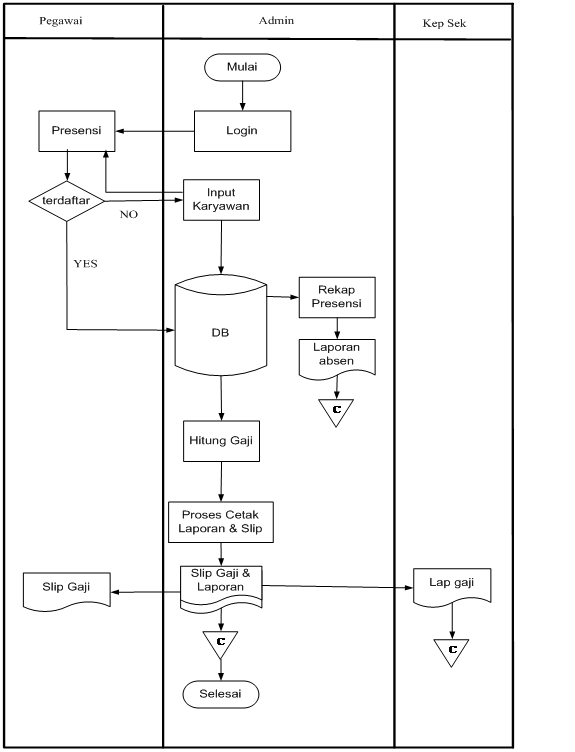
\includegraphics[width=0.7\textwidth]{gambar/1}  
 \caption{Flowchart Metode Penelitian}
\end{figure}

\section{Alat dan Bahan}
Dalam pelaksanaan dan penyusunan Laporan Tugas Akhir (TA) ini digunakan bahan dan alat sebagai berikut :

\vspace{-0.5cm}

\begin{enumerate}[a.]
\begin{singlespace}
\itemsep0em
\item Laptop/PC (2 unit),
\item Sistem Operasi (Windows 7),
\item Neatbean IDE 7.2 (Java),
\item Microsoft Visio 2010,
\item MySQL Workbench 6.0 (database),
\item Wifi/Modem (Koneksi Internet).
\end{singlespace}
\end{enumerate}

\section{Objek Penelitian}

Kegiatan pembuatan program aplikasi penggajian untuk guru ini mengambil lokasi di Yayasan TK/Paud Terpadu Al Mahrus
\subsection{Metode Pengumpulan Data}

Untuk menyelsaikan permasalahan yang ada, metode pengumpulan data yang dilakukan oleh penulis adalah dengan cara :

Metode ini yaitu dengan cara mengumpulkan dan meminta beberapa contoh dokumen atau data yang digunakan  dengan masalah yang diteliti. Adapun contoh yang penulis ambil seperti :
\begin{itemize}
\item[a.]	Dokumen data pegawai
\item[b.]   Data laporan presensi
\item[c.]	Slip gaji 
\item[d.]	Laporan gaji
\end{itemize}

Metode Wawancara (interview)

Metode interview ini yaitu dengan cara menanyakan beberapa pertanyaan yang berhubungan dengan topik yang dibahas kepada pihak-pihak yang bersangkutan yang terdiri dari :

\begin{itemize}


\item[a.]	Bagian Bendahara
Menanyakan sistem pembayaran dan perhitungan gaji serta menanyakan sistem pencatatan presensi.

\item[b.]	Bagian Kepala Sekolah
Menanyakan struktur organisasi yang ada di SMA Muhammadiyah 02 Wuluhan.

\item[c.]	Metode Observasi
Metode ini dengan meninjau dan mengamati secara langsung sistem yang sedang berjalan di sekolahan tersebut serta mencatat informasi yang terkait dengan sistem informasi penggajian yang selanjutnya akan dianalisis dan digunakan dalam pembuatan desain program Sistm Informasi Penggajian pada SMA Muhammadiyah 02 Wuluhan.

\item[d.]	Metode Pustaka
Metode mencatat yang berasal dari buku-buku yang ada hubungannya dengan obyek yang ditangani.
\end{itemize}
%-----------------------------------------------------------------
%Disini akhir masukan Bab
%-----------------------------------------------------------------

%-----------------------------------------------------------------
%Disini awal masukan untuk Daftar Pustaka
%-----------------------------------------------------------------
%%\nocite{Abel2010,Guerbas201350}
%%\bibliography{research-plan}
%%\bibliographystyle{plainnat}
\begin{thebibliography}{9}

\bibitem[satu(2014)]{satu01}
Al-Bahra Bin Ladjamudin. 2005. Analisis dan Desain Sistem Informasi. Tangerang : Graha Ilmu

\bibitem[dua(2014)]{dua02}
Hartono, Jogiyanto. 1999. Pengenalan Komputer : Dasar Ilmu Komputer, Pemrograman, Sistem Informasi dan Intelegensi Buatan. Yogyakarta : Andi Yoyakarta.

\bibitem[tiga(2014)]{tiga03}
Hartono,Jogiyanto. 1990. Analisis dan Disain Sistem Informasi. Yogyakarta: Andi Offset

\bibitem[empat(2014)]{empat04}
Hartono, Jogiyanto. 1989. Analisis dan Disain Sistem Informasi Pandekatan Terstruktur : Teori Dan Praktek Aplikasi Bisnis. Yogyakarta : Andi

\bibitem[lima(2014)]{lima05}
Huda, Miftakhul. Membuat Aplikasi Rental dengan Java dan MySql, Penerbit PT Elex Media Komputindo-Jakarta 2009.

\bibitem[enam(2014)]{enam06}
Kristanto, Andi. 2008. Perancangan Sistem Informasi. Yogyakarta : Gava Media

\bibitem[tujuh(2014)]{tujuh07}
Supardi, Yuniar. Semua Bisa Menjadi Programer Java – Study Case, Penerbit PT Elex Media Komputindo-Jakarta 2010.


\end{thebibliography}
\addcontentsline{toc}{chapter}{DAFTAR PUSTAKA}
%-----------------------------------------------------------------
%Disini akhir masukan Daftar Pustaka
%-----------------------------------------------------------------

\end{document}